\section{Findings}\label{sec:findings}

\subsection{Finding 1: winners' domains move in lockstep with the year's theme}

Figure~\ref{fig:themes} plots each examined winner's domain against its year.
The fit is essentially perfect: procurement tools win in procurement-themed
years, carbon tools in net-zero years, AI-for-excluded-groups in the AI era.
This is not necessarily judges ``choosing politics over quality'' --- entrants
self-select onto the theme, and the theme filters the pool before judges see
it. But it means \emph{no observed winner has ever won against the year's
current}. The theme is set to the presidential agenda by
design\cite{handbook}; the record confirms the design works.

\begin{figure}[htbp]
\centering
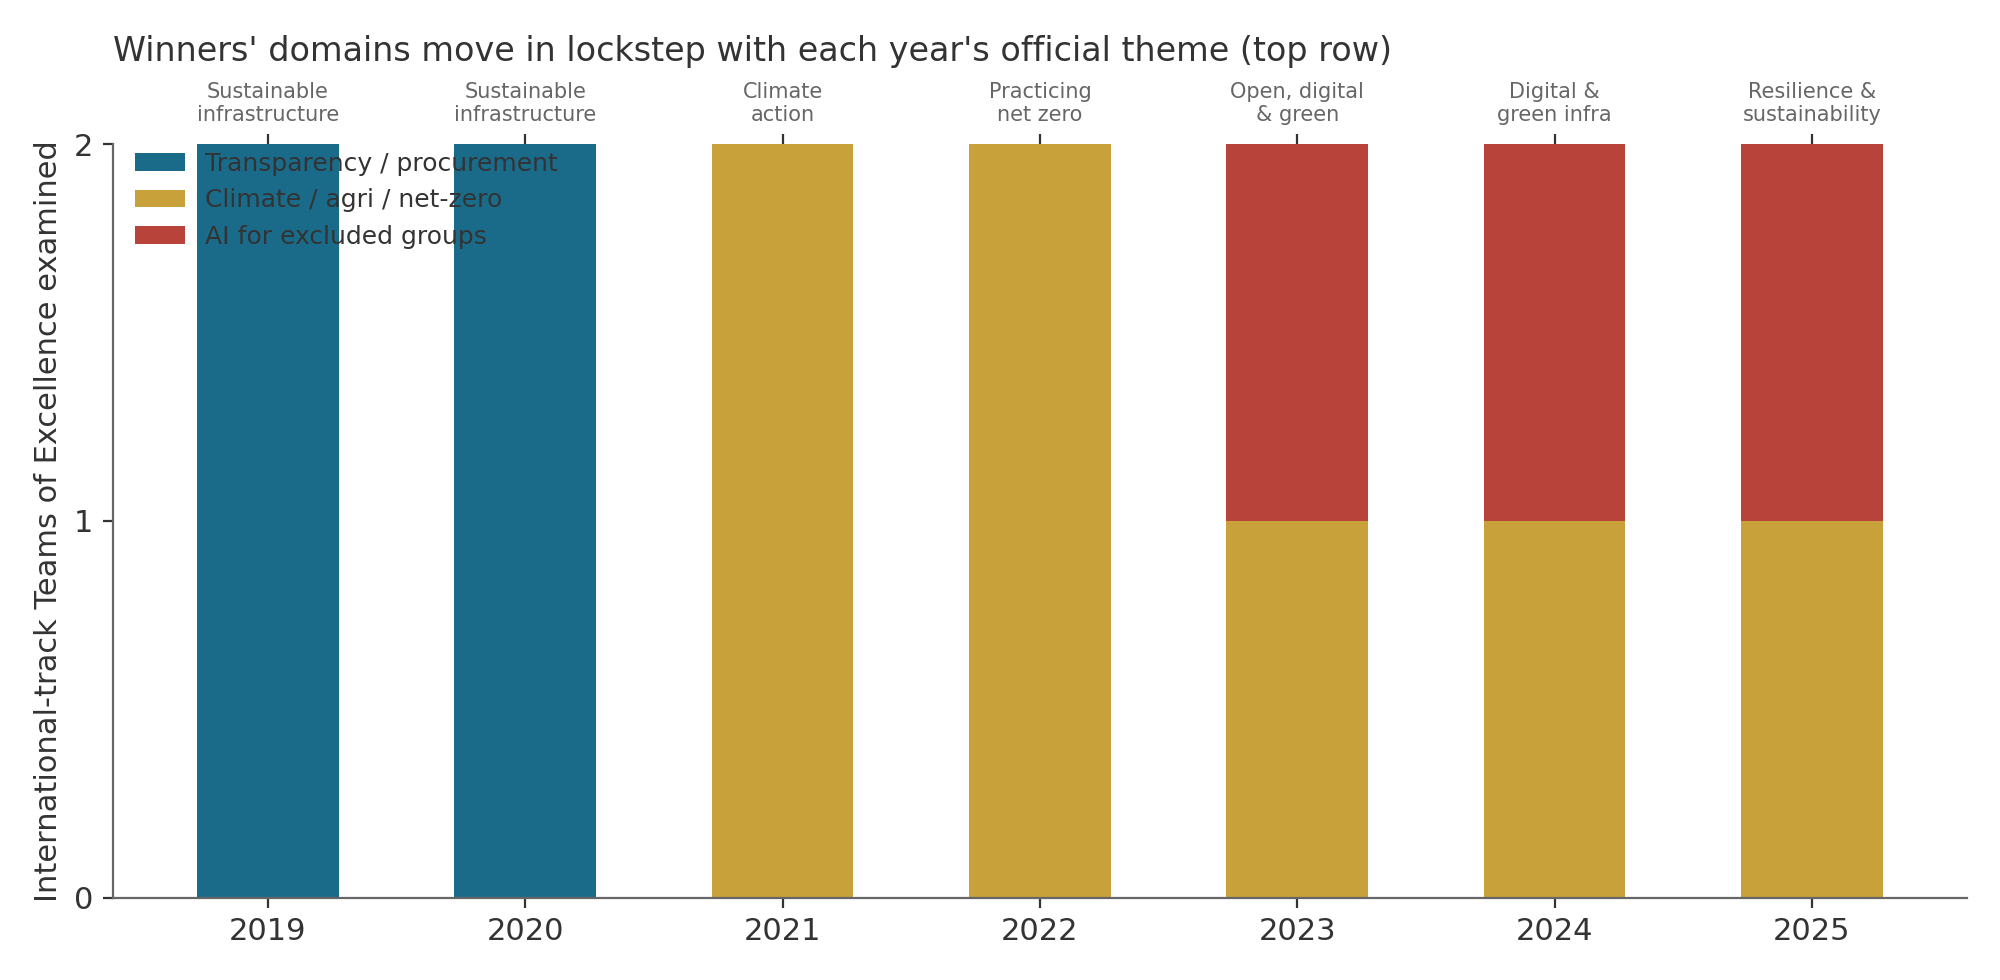
\includegraphics[width=0.95\textwidth]{chart6_themes.png}
\caption[Winners' domains vs.\ the year's official theme]{Domains of the 14
examined Teams of Excellence against each year's official theme (top row).
Sources: official press releases and history pages\cite{moda2023,moda2024,pres2025,hist2023,ocpfiscal}.}
\label{fig:themes}
\end{figure}

\subsection{Finding 2: half the winners did not start at the hackathon}

Of the fourteen examined entries, four were demonstrably pre-existing products
or platforms (SISOCS, 2014--15\cite{cost}; A/B Street, 2018\cite{abstreet};
HysonTech's aquaculture line\cite{hyson}; GreenHope's carbon
wallet\cite{greenhope}), and at least three more were new builds by existing
organizations (CivicDataLab's Fiscal Force\cite{ocpindia}; Sinar-backed
Cartelogy\cite{ocpcartel}; CropNow's NEST device team\cite{focuscrop}). For
the remaining seven we found no evidence either way
(Figure~\ref{fig:maturity}). The competition's own rules acknowledge this
reality: entries previously sold or awarded must be modified by at least
50\%\cite{handbook} --- a rule you only write when mature entries are common.
\textbf{Implication: ``hackathon'' is a misnomer; this is a showcase for
projects that already exist at least in embryo, judged partly on how real
they already are.} That is consistent with a rubric that puts Feasibility
(40\%) above Innovation (30\%)\cite{handbook}.

\begin{figure}[htbp]
\centering
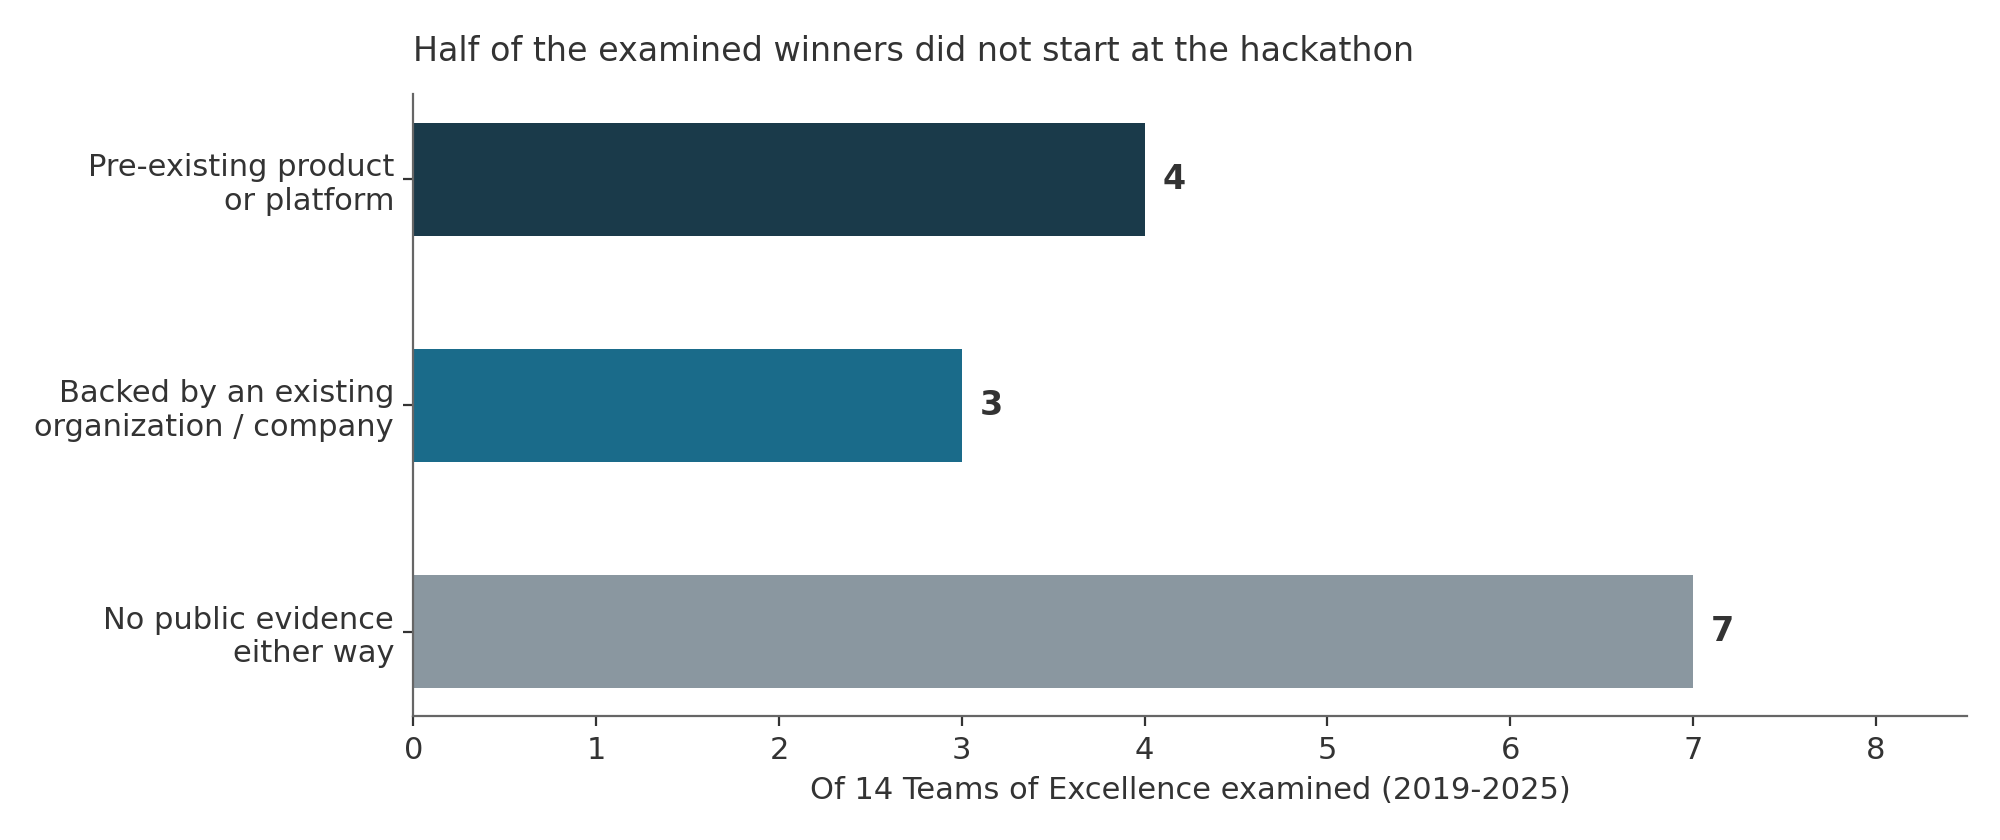
\includegraphics[width=0.95\textwidth]{chart7_maturity.png}
\caption[Maturity of winning entries at the time of winning]{Maturity of the
examined winners at the time of winning. ``No public evidence either way''
means our searches found neither a pre-existing product nor proof the build
began at the competition.}
\label{fig:maturity}
\end{figure}

\subsection{Finding 3: the afterlife record is split exactly in half}

Seven of fourteen winners show documented post-competition activity: CoST's
platform still discloses projects at national scale\cite{cost}; CivicDataLab's
hackathon index became a formal multi-state partnership\cite{ocpindia}; A/B
Street continues, diminished, through its creator's
consultancy\cite{abinterview}; HysonTech and GreenHope operate
commercially\cite{hyson,greenhope}; CropNow and Beyond Hearing were presented
by MODA itself in 2026 as progressing implementations\cite{moda2026}. The
other seven --- Cartelogy, Learning Man, Office Farmers, BRSDM@Er-Lin,
B.E.N.Z., Re-Fill City, MooApps --- left no public trace we could find
(Figure~\ref{fig:afterlife}). The pattern within the split is sharper than the
split itself: \textbf{every winner with a documented afterlife had an
institution, company, or funded program behind it; every winner without one
was, as far as the record shows, a team formed around a competition.} The
Presidential Hackathon amplifies projects; the evidence does not show it
sustaining them. (MODA's own claim that winning proposals are implemented and
tracked\cite{moda2026,pmc} is documented mainly through domestic-track
examples, such as the emergency-response system that became
policy\cite{pmc}.)

\begin{figure}[htbp]
\centering
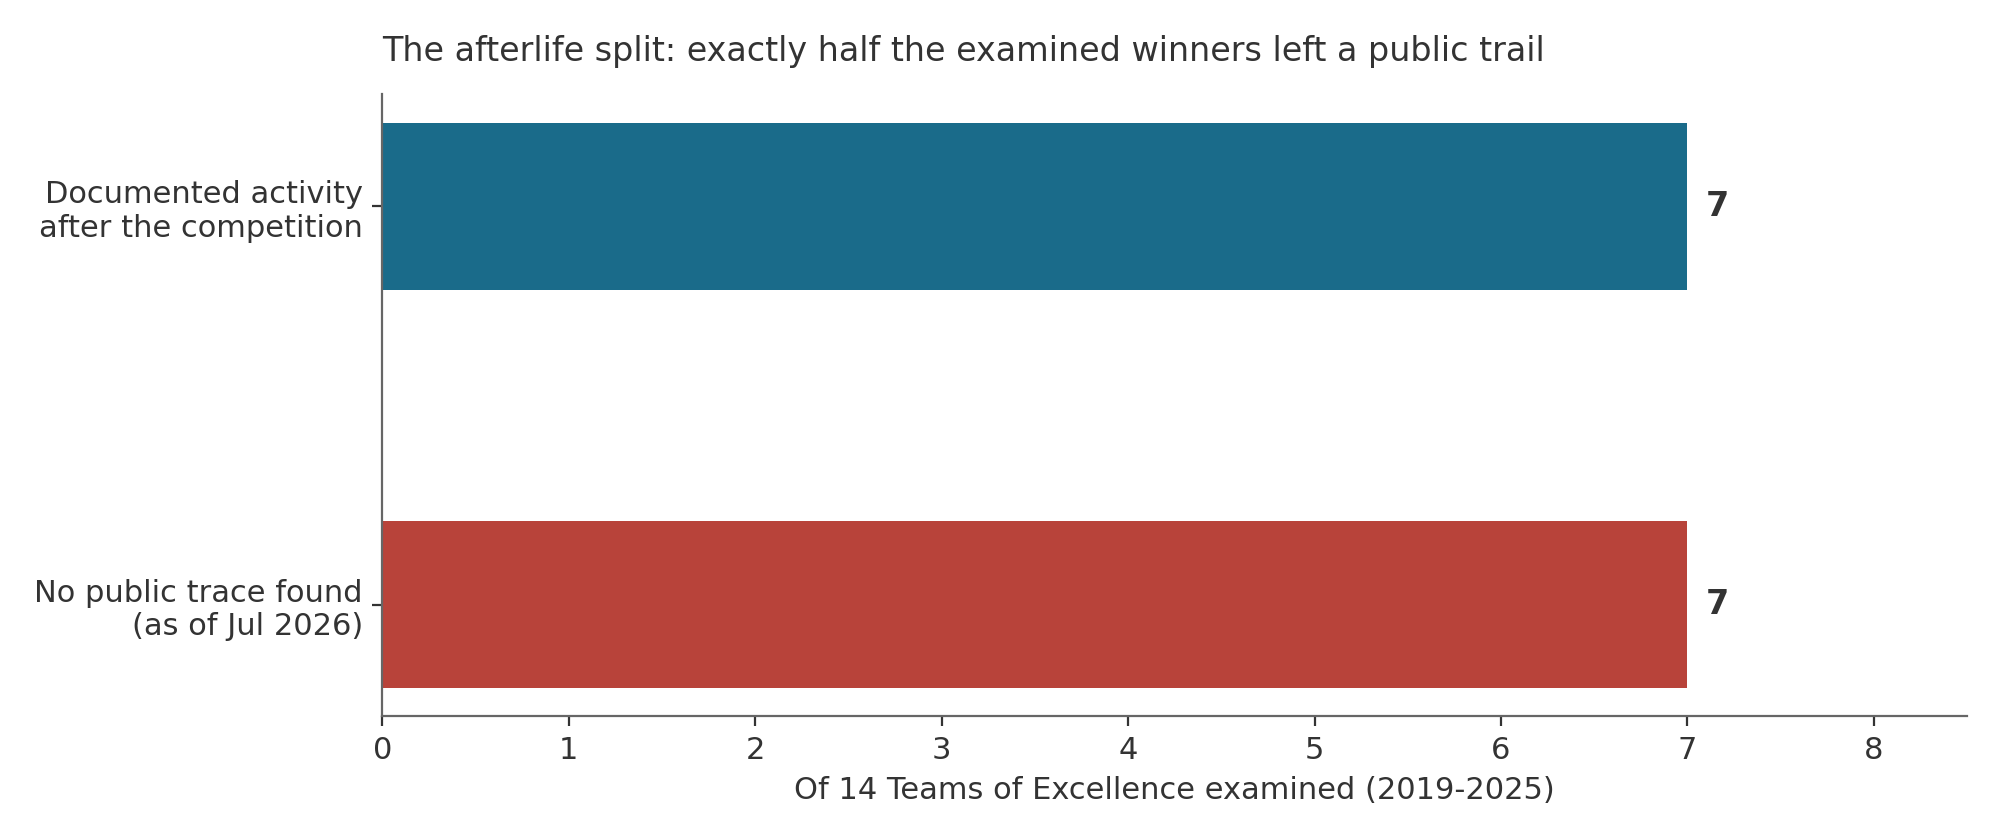
\includegraphics[width=0.95\textwidth]{chart8_afterlife.png}
\caption[Post-competition traces of the 14 winners]{Post-competition public
traces of the examined winners, as of July 2026. ``No public trace found'' is
weak evidence --- teams may continue privately --- and is reported as such.}
\label{fig:afterlife}
\end{figure}

\subsection{Finding 4: the diplomatic pattern is visible and unhidden}

India appears among the winners in four of seven editions (Fiscal Force 2020,
B.E.N.Z. 2022, HysonTech's co-team 2023, CropNow 2025); the 2025 award
ceremony was attended by the India--Taipei Association's acting
chairperson\cite{focuscrop}; 2019's winner came from Honduras, then a
diplomatic ally, via a program co-branded with the World Bank\cite{cost}. The
International Track is, openly, an instrument of Taiwan's ``Taiwan Can Help''
outreach --- multinational teams are a scored expectation (at least one
non-ROC national is mandatory\cite{handbook}). This does not diminish the
winners; it describes the selection environment honestly: \textbf{a good
project that also serves Taiwan's international positioning is worth more, in
this arena, than a slightly better project that does not.}

\subsection{Finding 5: corrections to our own earlier files}\label{sec:corrections}

Re-verification caught two errors in this project's earlier research
documents, worth recording precisely because this review is meant to be
unbiased. (1) File~1 described 2022's B.E.N.Z. as ``AI applications deployed
in smart agriculture ecosystems''; the competition's own history page
describes a GIS-based tree-placement and urban-forest project\cite{hist2023}
--- less AI, more geography. (2) The same file listed Cartelogy as a 2019
Team of Excellence; the Open Contracting Partnership's contemporaneous account
says ``top 2 teams out of almost 30 applicants''\cite{ocpcartel}, while a
Malaysian government portal celebrates a different Malaysian team
(``Mentadak'') as award-winning --- the precise 2019 honor roll is thus
partially ambiguous in accessible English sources, and we flag rather than
resolve it. Neither correction changes the structural findings; both
illustrate how easily secondary summaries drift toward the more flattering,
more AI-flavored version of events.
